\documentclass[10pt,landscape]{article}
\usepackage{multicol}
\usepackage{calc}
\usepackage{ifthen}
\usepackage[landscape]{geometry}
\usepackage{hyperref}
\usepackage{graphicx}
\usepackage{breqn}
\usepackage{amsmath,amssymb}
\usepackage{algorithm2e}
\setlength{\algomargin}{0.5em}
%\RestyleAlgo{tworuled}
\usepackage{float}
\usepackage{changepage}
\usepackage{enumitem}
\usepackage{tikz}
\newcommand*\circled[1]{\tikz[baseline=(char.base)]{
            \node[shape=circle,draw,inner sep=2pt] (char) {#1};}}
            \documentclass{article}
\usepackage[thinlines]{easytable}



% This sets page margins to .5 inch if using letter paper, and to 1cm
% if using A4 paper. (This probably isn't strictly necessary.)
% If using another size paper, use default 1cm margins.
\ifthenelse{\lengthtest { \paperwidth = 11in}}
        { \geometry{top=.5in,left=.5in,right=.5in,bottom=.5in} }
        {\ifthenelse{ \lengthtest{ \paperwidth = 297mm}}
                {\geometry{top=1cm,left=1cm,right=1cm,bottom=1cm} }
                {\geometry{top=1cm,left=1cm,right=1cm,bottom=1cm} }
        }

% Turn off header and footer
\pagestyle{empty}


% Redefine section commands to use less space
\makeatletter
\renewcommand{\section}{\@startsection{section}{1}{0mm}%
                                {-1ex plus -.5ex minus -.2ex}%
                                {0.5ex plus .2ex}%x
                                {\normalfont\large\bfseries}}
\renewcommand{\subsection}{\@startsection{subsection}{2}{0mm}%
                                {-1explus -.5ex minus -.2ex}%
                                {0.5ex plus .2ex}%
                                {\normalfont\normalsize\bfseries}}
\renewcommand{\subsubsection}{\@startsection{subsubsection}{3}{0mm}%
                                {-1ex plus -.5ex minus -.2ex}%
                                {1ex plus .2ex}%
                                {\normalfont\small\bfseries}}
\makeatother

% Define BibTeX command
\def\BibTeX{{\rm B\kern-.05em{\sc i\kern-.025em b}\kern-.08em
    T\kern-.1667em\lower.7ex\hbox{E}\kern-.125emX}}

% Don't print section numbers
\setcounter{secnumdepth}{0}


\setlength{\parindent}{0pt}
\setlength{\parskip}{0pt plus 0.5ex}

\DeclareMathOperator*{\argmax}{argmax}

%----------------------------------------------------------------------------------------
%----------------------------------------------------------------------------------------
%----------------------------------------------------------------------------------------
%----------------------------------------------------------------------------------------

\begin{document}

\raggedright
\footnotesize
\begin{multicols}{3}

% multicol parameters
% These lengths are set only within the two main columns
%\setlength{\columnseprule}{0.25pt}
\setlength{\premulticols}{1pt}
\setlength{\postmulticols}{1pt}
\setlength{\multicolsep}{1pt}
\setlength{\columnsep}{2pt}

\begin{center}
     \Large{Reinforcement Learning Cheat Sheet} \\
\end{center}

%----------------------------------------------------------------------------------------
%	MDP
%----------------------------------------------------------------------------------------


\section{Markov Decision Process}
A tuple $(T, S, (A_s, p(\cdot | s,a), r_t(s,a), 1 \leqslant t \leqslant T, s \in S, a \in A_s))$ where:
\begin{equation*}
        \begin{array}{l}
         \text{finite set of states : }
                s \in S \\
         \text{finite set of actions : }
        a \in A \\
                 \text{state transition probabilities : }\\
        p(s' | s, a) = Pr \{S_{t + 1} = s' | S_t = s, A_t = a \} \\
                \text{reward for a given state-action pair : }\\
        r_t(s, a) \in \mathbb{R}  \\
        \end{array}
\end{equation*}
We seek to maximize : \\
if T is finite : expected total reward
$$R = \mathbb{E} \left [\sum_{t=1}^{T} r_t(s_t, a_t) \right ]$$
if T is infinite : discounted reward (typically $\lambda = 0,9$)
$$R = \underset{T \rightarrow \infty}{\textup{lim}}\mathbb{E} \left [\sum_{t=1}^{T} \lambda^{t-1} r_t(s_t, a_t) \right ]$$
We can then define the expected return at time t :
\begin{equation*}
    \begin{array}{1}
         R_t = \mathbb{E} \left [\sum_{t'=t}^{T} r_{t'}(s_{t'}, a_{t'}) \right ] \\
        \text{or} \\
        R_t = \underset{T \rightarrow \infty}{\textup{lim}}\mathbb{E} \left [\sum_{t'=t}^{T} \lambda^{t'-1} r_{t'}(s_{t'}, a_{t'}) \right ]
    \end{array}
\end{equation*}

%----------------------------------------------------------------------------------------
%	Value Function
%----------------------------------------------------------------------------------------


\section{Value Function}
Value function describes \emph{how good} it is to be in a specific state $s$ under a certain policy $\pi$. For MDP:
\begin{equation*}
V^{\pi}(s) = \mathbb{E} \left [ R^\pi | s_1^\pi = s \right ]
\label{eq: value_func}
\end{equation*}

Informally, it is the expected return when starting from $s$ and following $\pi$

\subsection{Optimal}

\begin{equation*}
V^*(s) = \sup\limits_{\pi} V_\pi(s)
\label{eq: value_optimal}
\end{equation*}


%----------------------------------------------------------------------------------------
%	Q Function
%----------------------------------------------------------------------------------------

\section{Action-Value (Q) Function}
We can also denote the expected reward for state, action pairs.
\begin{equation*}
Q^{\pi}(s, a) = \mathbb{E} \begin{bmatrix} R^\pi | s_1^\pi = s, a_1^\pi = a \end{bmatrix}
\label{eq: q_func}
\end{equation*}

Complexity of evaluating the Q-function with finite T : $A^TS^{T+1}$, i.e. the number of possible trajectories
\subsection{Optimal}
The optimal value-action function:
\begin{equation*}
Q^*(s,a) = \sup\limits_{\pi} Q^\pi(s,a)
\label{eq: action_value_optimal}
\end{equation*}
Using this new notation we can redefine $V^*$, using $S^*(s,a)$ :
\begin{equation*}
V^*(s) = \max\limits_{a \in A_s} Q^{*}(s,a)
\end{equation*}
Intuitively, the above equation express the fact that the value of a state under the optimal policy \textbf{must be equal} to the expected return from the best action from that state.

%----------------------------------------------------------------------------------------
%	Bellman
%----------------------------------------------------------------------------------------


\section{Bellman's Equations}

\subsection{Bellman's Optimality Equation}

\begin{equation*}
    V^*(s) = \max\limits_{a \in A_s} \underbrace{ \left [ r(s,a) + \lambda \sum_{j} p(j|s,a)V^*(j) \right ]}_{Q(s,a)}
\end{equation*}

\subsection{Bellman's Expectation Equation}

\begin{equation*}
    V^\pi(s) = \mathbb{E}_\pi \left [ r^\pi(s) + \lambda \sum_{j} \pi(j|s)V^\pi(j) \right ]
\end{equation*}


%----------------------------------------------------------------------------------------
%	Contraction Mapping
%----------------------------------------------------------------------------------------

\section{Contraction Mapping}

This part is a preliminary to Dynamic Programming

\subsection{Definition}

Let $(X, d)$ be a metric space and $f: X \rightarrow X$. We say that $f$ is a
\emph{contraction} if there is a real number $k \in [0, 1[$ such that \begin{equation*}
    d(f(x), f(y)) \leq k d(x, y)
\end{equation*}

for all $x$ and $y$ in $X$, where the term $k$ is called a \emph{Lipschitz coefficent} for $f$.

\subsection{Contraction Mapping theorem}

Let $(X,d)$ be a complete metric space and let $f: X \rightarrow X$ be a contraction.
Then there is one and only one fixed point $x^\ast$ such that
\begin{equation*}
 f(x^\ast) = x^\ast
\end{equation*}

Moreover, if $x$ is any point in $X$ and $f^n(x)$ is inductively defined by
$f^2(x) = f(f(x))$, $f^3(x)=f(f^2(x))$, \ldots, $f^n(x)=f(f^{n−1}(x))$,
then $f^n(x) \rightarrow x^\ast$ as $n \rightarrow \infty$. This theorem guarantees
a unique optimal solution for the dynamic programming algorithms detailed below.


%----------------------------------------------------------------------------------------
%	DP
%----------------------------------------------------------------------------------------

\section{Dynamic Programming}
When we know the MDP, we can use Bellman's equation to find the optimal policy by just \emph{planning} (no learning)


\subsection{Value Iteration}
\begin{algorithm}[H]
  \SetKwInOut{Output}{output}
 Initialize $V_0(s) \in \mathbb{R}, \text{ e.g } V_0(s) = 0$ \\
 \While{$ \left \| V_n - V_{n-1} \right \| \geqslant \epsilon$}{
  \ForEach{$s \in S$} {
        $V_{n+1}(s) = \max\limits_a \left [ r(s,a) + \lambda \sum\limits_{j} p(j | s, a) V_n(j) \right ]$ \\
  }
 }
 \Output{Probably Approximately Correct (PAC) optimal value function $V \approx V^*$}
 \caption{Value Iteration}
 \medskip
 \end{algorithm}
 \medskip
 We can then derive a PAC optimal policy $\pi \approx \pi^*$ such that $$\pi(s) \in \argmax\limits_a  [ r(s,a) + \lambda \sum\limits_{j} p(j | s, a) V_n(j) ]$$
 VI converges almost surely to an $\epsilon$-optimal policy with complexity $\Theta(S^2A)$ for each iteration


\subsection{Policy Iteration}
Needs more steps but computes directly the optimal policy and is quicker than Value Iteration most of the time.

\subsubsection{Howard's Policy Iteration}
\begin{algorithm}[H]
\SetAlgoLined
\SetKwInOut{Output}{output}
 Initialize $V(s) \in \mathbb{R}, \text{e.g } V(s) = 0$, $\pi(s) \in A_s$  for all $s \in S$\\
 \While{$\pi_n \neq \pi_{n-1}$}{
 1. Policy Evaluation \\
 
  \ForEach{$s \in S$} {
        $ V^\pi_n(s)= r^\pi(s) + \lambda \sum_{j} \pi(j|s)V^\pi_n(j) $
        }

 
 2. Policy Improvement \\
  \ForEach{$s \in S$} {
        $ \pi_{n+1}(s) = \argmax\limits_a \left [r(s,a) + \lambda \sum_j p(j|s,a) V^\pi_n(j) \right ] $
  }
}
\Output{PAC optimal value function and policy $V \approx V^*$ and $\pi \approx \pi^*$}
\caption{Howard's Policy Iteration}
 \medskip
\end{algorithm}

\subsubsection{Simplex Policy Iteration}
\begin{algorithm}[H]
\SetAlgoLined
\SetKwInOut{Output}{output}
 Initialize $V(s) \in \mathbb{R}, \text{e.g } V(s) = 0$, $\pi(s) \in A_s$  for all $s \in S$\\
 \While{$\pi_n \neq \pi_{n-1}$}{
 1. Policy Evaluation \\
 
  \ForEach{$s \in S$} {
        $ V(s)= \max\limits_{a \in A_s} \left [r(s,a) + \lambda \sum_j p(j|s,a) V^\pi_n(j) \right ] $\\
        Choose $s_0 \in \argmax\limits_{s \in S} (V(s) - V_n^\pi(s))$
        }

 
 2. Policy Improvement \\
  \ForEach{$s \in S \backslash s_0$} {
    $ \pi_{n+1}(s) = \pi_n(s) $
  }
  $ \pi_{n+1}(s_0) = \argmax\limits_{a \in A_{s_0}} \left [r(s_0,a) + \lambda \sum_j p(j|s_0,a) V^\pi_n(j) \right ] $
}
\Output{PAC optimal value function and policy $V \approx V^*$ and $\pi \approx \pi^*$}
\caption{Simplex Policy Iteration}
 \medskip
\end{algorithm}

Both of the above-mentioned versions converge with complexity $\Theta(S^\omega) + \Theta(S^2A)$ per iteration. Howard's and Simplex PI require respectively  $\mathcal{O}(\frac{A}{1-\lambda}\log{\frac{1}{1-\lambda}})$ and $\mathcal{O}(\frac{AS}{1-\lambda}\log{\frac{1}{1-\lambda}})$ iterations to converge (HPI is better with large state-spaces)

\end{multicols}
 
 
 
 
 
 
 
 
 
 
 
 
 
\newpage

\begin{multicols}{3}

%----------------------------------------------------------------------------------------
%   A few definitions
%----------------------------------------------------------------------------------------


\section{A few definitions}

\subsection{Model-free vs Model-based}
In Model-based methods (e.g. Dynamic Programming), we have complete knowledge of the model of the environment, contrary to Model-free methods (e.g. Monte Carlo). \\
\begin{array}{ccc}
    & \textbf{Model-based} & \textbf{Model-free} \\
    \text{Transitions/Rewards are} & \textbf{known} & \textbf{unknown}\\
    \text{Can predict without action} & \textbf{yes} &  \textbf{no} \\
    \text{Type of strategy} & \textbf{Planning} &  \textbf{Learning}
\end{array}

\subsection{On-policy vs Off-policy}

In On-policy learning (e.g. SARSA) the agent learns the value of the policy being carried out by the agent. \\In Off-policy learning (e.g. Q-Learning), the learning process is independent of the agent's actions, which are sampled from a \textbf{behavior policy}.

\subsection{Prediction vs Control}

In prediction tasks, given a policy, we want to compute how well it performs, while control tasks seek to find the optimal policy.

\subsection{Stationary vs Non-Stationary}

An environment is stationary if the transitions and rewards don't change over time. Non-stationary environments are beyond the scope of standard RL methods, except when the environment evolves slowly enough.


%----------------------------------------------------------------------------------------
%	Monte carlo
%----------------------------------------------------------------------------------------


\section{Monte Carlo Methods}
In Monte Carlo (MC) methods, we evaluate policies through sampling : the value being considered as the mean return. MC is Model-free, and on-policy. MC learns from complete episodes (no bootstrapping), and consequently all episodes must terminate.\\
\medskip
To implement it for control tasks, we use a MC Policy Evaluation, and add a Policy Improvement (e.g. $\epsilon$-greedy)

 \medskip
\begin{algorithm}[H]
 Initialize $Q(s,a) = 0$, $\pi(s) \in A_s$  for all $s \in S, a \in A_s$\\
 \ForEach{episode $1\leqslant i \leqslant n$}{
    1. Monte-Carlo Evaluation\\
    Sample a full trajectory $\tau_i = ((s_{1,i}, a_{1,i}, r_{1,i}), ..., (s_{T_i, i}, a_{T_i, i}, r_{T_i, i}))$ from $\pi$ \\
    $R = 0$\\
    \ForEach{t in $T_i, T_{i-1}, ..., 1$}{
        $R = r_{t,i} + \lambda R$\\
        \If{$s_{t,i}$ \textup{ is not visited later}}{
            $Q^{(i)}(s_{t,i}, a_{t,i}) = Q^{(i-1)}(s_{t,i}, a_{t,i}) + \frac{1}{i} \left (R - Q^{(i-1)}(s_{t,i}, a_{t,i}) \right)$
        }
    }
    2. $\epsilon$-greedy Policy Improvement\\
    \ForEach{$s$ \textup{in the episode}}{
        $\pi(s) = \left\{\begin{matrix}
\argmax\limits_a Q(s,a) & $w.p. $ 1 - \epsilon\\ 
\textup{uniform}(A_s) & $w.p. $ \epsilon
\end{matrix}\right.$
    }
 }
\caption{First-visit Monte Carlo Control}
\end{algorithm}
% }
For non-stationary problems, the Monte Carlo estimate for, e.g, $Q$ is:
\begin{equation*}
Q(s_t, a_t) \leftarrow Q(s_t, a_t) + \alpha \begin{bmatrix}
        R - Q(s_t, a_t)
\end{bmatrix}
\end{equation*}
Where $\alpha$ is the learning rate, quantifying how much we want to forget about past experiences.


%----------------------------------------------------------------------------------------
%	Stochastic Approximation
%----------------------------------------------------------------------------------------

\section{Stochastic Approximation}
This part is a preliminary to Temporal Difference.

\subsection{Robbins-Monro}
To find the root $x^* \in \mathbb{R^d}$ of a continuous function $h$ when we observe $Y \: / \: \mathbb{E}[Y(x)] = h(x)$
 \medskip
\begin{algorithm}[H]
    Initialize $x^*_{(0)} \in \mathbb{R^d}$\\
    \For{$k \geqslant 0$}{
        $x^*_{(k+1)} = x^*_{(k)} - \alpha_k Y(x^*_{(k)})$
    }
\caption{Robbins-Monro (RM)}
\end{algorithm}

($h$ must verify $\exists \beta >0 / \forall x \in \mathbb{R}^d, h(x)(x-x^*) \geqslant \beta \left \| x - x^* \right \|^2$)

\subsection{SA for extrema localisation}
If we use $x(t_k) = x^*_{(k)}$ with $t_k = \sum_{i=1}^{k-1} \alpha_i$ (i.e. $\alpha_k = t_k-t_{k-1}$), we can use the RM algorithm :
$$ \frac{x^*_{(k+1)} - x^*_{(k)}}{\alpha_k} = \underbrace{\frac{x(t_{k+1}) - x(t_{k})}{t_{k+1} - t_k}}_{\rightarrow \overset{\cdot}{x}(t_k)  \textup{ as }k \rightarrow \infty} =  Y(x(t_{k}))$$

Under certain assumptions, we have that
$$\lim_{k \rightarrow \infty} x^{(k)} = x^* $$ where $x^*$ is the only globally stable point of $\overset{\cdot}{x} = h(x)$.\\
By adding 2 more assumptions, we can derive an asynchronous version (only a subset of coordinates of $x^{(k)}$ are updated at each iteration), which can be used for Temporal Difference Learning.


%----------------------------------------------------------------------------------------
%	Temporal Difference
%----------------------------------------------------------------------------------------


\section{Temporal Difference}
Temporal Difference (TD) methods learn directly from raw experience without a model of the environment's dynamics. TD substitutes the expected discounted reward $R_t$ from the episode with an estimation:

$\begin{array}{cc}
    \textbf{MC Update} & $V(s_t) \leftarrow V(s_t) + \alpha_t \left [\underbrace{R_t}_{target} - V(s_t) \right ]$ \\
    \textbf{TD Update} & $V(s_t) \leftarrow V(s_t) + \alpha_t \left [\underbrace{r_t + \lambda V(s_{t+1})}_{target} - V(s_t) \right ]$ 
\end{array}$

TD methods are Model-free, with bootstrapping (i.e. only the current estimate is used as target).\\
TD presents the advantage of being adapted to continuing environments where some episodes never terminate, thanks to \textbf{on-line learning}, i.e. update after every step. Q-Learning and SARSA are the most common TD methods.

\subsection{SARSA}
SARSA (State-Action-Reward-State-Action) applies directly the above-mentioned principle.

\begin{algorithm}[H]
 Initialize $Q(s,a) = 0$, $\pi(s) \in A_s$  for all $s \in S, a \in A_s$\\
 \ForEach{episode $1\leqslant i \leqslant n$}{
    \ForEach{step $t$ until end}{
        Choose $a_t$ $\epsilon$-greedily\\
        Observe $r_t, s_{t+1}, a_{t+1}$\\
        $Q^{(t+1)}(s_t, a_t) = Q^{(t)}(s_t, a_t) + \alpha \left [ r_t + \lambda Q^{(t)}(s_{t+1}, a_{t+1}) - Q^{(t)}(s_t, a_t) \right ]$
    }
 }
\caption{SARSA}
\end{algorithm}


\subsection{Q-Learning}
In Q-Learning, the target is different  since it uses the optimal action at state $s_{t+1}$

\begin{algorithm}[H]
 Initialize $Q(s,a) = 0$, $\pi(s) \in A_s$  for all $s \in S, a \in A_s$\\
 \ForEach{episode $1\leqslant i \leqslant n$}{
    \ForEach{step $t$ until end}{
        Choose $a_t$ $\epsilon$-greedily\\
        Observe $r_t, s_{t+1}$\\
        $Q^{(t+1)}(s_t, a_t) = Q^{(t)}(s_t, a_t) + \alpha \left [ r_t + \lambda \max\limits_{b \in A} Q^{(t)}(s_{t+1}, b) - Q^{(t)}(s_t, a_t) \right ]$
    }
 }
\caption{Q-Learning}
\end{algorithm}

\subsection{Comparison of SARSA and Q-Learning}

SARSA is on-policy while Q-Learning is off-policy.\\
\medskip
Indeed, Q-Learning learns the true Q-function of the optimal policy, not the Q-function of the behavior policy.\\
\smallskip
Meanwhile SARSA learns the Q-function of the behavior policy including the $\epsilon$-greedy exploration phase.\\
\medskip
This implies that SARSA is "safer" since it takes into account the random exploration of the agent, which may be better if the agent is used while learning in some cases:


\centering
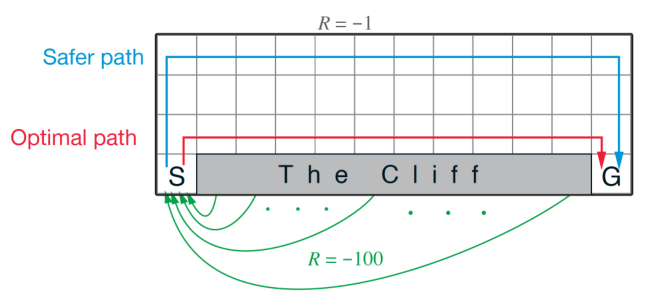
\includegraphics[width=0.3\textwidth]{cliff.PNG}
\caption{SARSA tends to follow a safer path}

\end{multicols}
 
 
 
 
 
 
 
 
 
 
\newpage

\begin{multicols}{3}

%----------------------------------------------------------------------------------------
%	Policy Gradients
%----------------------------------------------------------------------------------------

\section{Policy Gradients}

\subsection{Introduction}
The objective is to maximize the value function from the first state. To do so we parameterize the policy such that $\pi_\theta(s,a)$ is the probability of taking action $a$ in state $s$ and is defined with respect to $\theta \in \mathbb{R}^n$.\\
If we note a trajectory as $\tau = (s_1,a_1, ..., s_T, a_T)$ with $s_1$ sampled from a distribution $p$, we seek to maximize $$ J(\theta) =\mathbb{E}_{s_1 \sim p} \left [ V^{\pi_\theta}(s_1) \right ] $$ with  $$V^{\pi_\theta}(s) = \mathbb{E}_{\pi_\theta} \left [ \sum_{t=1}^{T} r(s_t, a_t) \mid s_1 = s \right ] $$

\medskip

To maximize $J$ and find the optimal policy $\pi_{\theta^*}(s,a)$, we apply gradient descent on theta, i.e. we iteratively update theta : $$ \theta_{k+1} = \theta_k + \alpha \nabla_\theta J(\theta_k) $$

\subsection{The Policy Gradient Theorem}

The PG Theorem gives an expression of the gradient of $J$. Since $J(\theta)$ can be equivalently written as 
$$ J(\theta) = \sum_\tau \pi_\theta(\tau) R(\tau) $$ 
By using the log derivative trick we get 
$$ \nabla J(\theta) = \sum_\tau \pi_\theta (\tau) \times \left ( \nabla \log \pi_\theta (\tau) R(\tau) \right )$$
$$ \Leftrightarrow \nabla J(\theta) = \mathbb{E}_{\pi_\theta} \left [ \nabla \log \pi_\theta (\tau) R(\tau) \right ]$$
and finally
$$ \nabla J(\theta) = \mathbb{E}_{\pi_\theta} \left [ \left ( \sum_{t=1}^T \nabla \log \pi_\theta (s_t, a_t) \right ) \left ( \sum_{t=1}^T r(s_t, a_t) \right ) \right ]$$

\subsection{REINFORCE}

REINFORCE is the direct application of the PG Theorem with Monte-Carlo philosophy. It only works with MC Rollouts, i.e. full trajectories, and thus requires finite episodes.

\begin{algorithm}[H]
 Initialize $\theta^{(0)} \in \mathbb{R}^n$\\
 \ForEach{episode $1\leqslant k \leqslant n$}{
    Generate $\tau_k = (s_{1,k}, a_{1,k}, r_{1,k}, ..., s_{T_k,k}, a_{T_k,k}, r_{T_k,k})$\\
    $\theta^{(k+1)} = \theta^{(k)} + \alpha_k \left ( \sum_{t=1}^{T} \nabla \log \pi_\theta ( s_{t,k}, a_{t,k}) \right ) \left ( \sum_{t=1}^{T} r_{t,k} \right )$
 }
\caption{REINFORCE}
\end{algorithm}


\subsection{Variance reduction}
To reduce the variance of the estimator used in REINFORCE and make the learning process faster and more stable, we can :\\

\begin{enumerate}[label=\protect\circled{\arabic*}]
\item Compute several trajectories and average the gradient estimator.
\item Use Reward-to-go : We use only the rewards from the future, i.e. the update becomes $$ \theta \leftarrow \theta + \alpha \sum_{t=1}^{T} \nabla \log \pi_\theta ( s_t, a_t)  \sum_{u=t}^{T} r_u $$
This is valid because of the Expected Grad-Log-Prob (EGLP) lemma (obtained with the log derivative trick) : 
    $$ \mathbb{E}_{\pi_\theta} \left [ \nabla \log \pi_\theta(s_t, a_t) r_u \right ] = 0$$
\item Add a baseline : $R(\tau) \rightarrow R(\tau) - b$. \\Examples of baselines :
\begin{itemize}[leftmargin=*]
    \item Natural (average of episodes): $b = \frac{1}{n} \sum_{i=1}^n \sum_{t=1}^T r(s_{t,i}, a_{t,i})$
    \item Variance-optimal: $b = \min \textup{Var}(X) = \frac{\mathbb{E}_{\pi_\theta} \left [ (\nabla_\theta \log \pi_\theta (\tau))^2 R(\tau) \right ]}{\mathbb{E}_{\pi_\theta} \left [ (\nabla_\theta \log \pi_\theta (\tau))^2 \right ]}$
    \item Reward-to-go : $b =\frac{1}{n} \sum_{i=1}^n \sum_{t=\mathbf{u}}^T r(s_{t,i}, a_{t,i}) $\\
    \item Value function (most common) : $b = V^{\pi_\theta}(s_t)$, often approximated by a neural network $V_\Phi (s_t)$ trying to minimize the MSE :
    $$\Phi_k = \textup{arg}\min\limits_\Phi \mathbb{E}_{s_t,\widehat{R}_t \sim \pi_k} \left [ (V_\Phi(s_t) - \widehat{R}_t)^2 \right ]$$
\end{itemize}
\end{enumerate}\\

\subsection{Vanilla Policy Gradient}

It can be shown that replacing $R(\tau)$ in the PG Theorem by $Q^{\pi_\theta}(s_t, a_t)$ is also a valid choice. If we add the value function as baseline we obtain for the PG update :
$$ \theta \leftarrow \theta + \alpha \sum_{t=0}^T \nabla \log \pi_\theta (s_t, a_t) A^{\pi_\theta}(s_t, a_t) $$

with $ A^{\pi_\theta}(s, a) = Q^{\pi_\theta}(s, a) - V^{\pi_\theta}(s)$ being the Advantage function, intuitively representing how much better or worse on average a certain action is compared to other actions (relatively to the current policy). Most of the time we don't compute the true value of $A$ but instead use a critic neural network $A_\Phi $ (see Actor-Critic methods).\\

\medskip 
A REINFORCE algorithm with averaging of several trajectories, Reward-to-go, and the use of the advantage function is called Vanilla Policy Gradient (VPG).\\


\begingroup
    \fontsize{5pt}{6pt}
        \textit{See also TRPO, PPO, DDPG, T3C}
\endgroup


%----------------------------------------------------------------------------------------
%	Function Approximation
%----------------------------------------------------------------------------------------

\section{Function Approximation}
Computing the true value of functions such as $V$ or $Q$ is costly: under the PAC framework, it scales as $S \times A$ where $S$ and $A$ are the dimension of respectively the state and action spaces. For continuous state-action spaces (like most real-world applications), it becomes infeasible.\\
Instead we use function approximation on parametrized value functions $V_\theta$ and $Q_\theta$, which requires modifying the update steps accordingly :

\medskip

\textbf{Monte-Carlo :}  $$\theta \leftarrow \theta + \alpha \left ( R - Q_\theta(s_t, a_t) \right ) \nabla_\theta Q_\theta(s,a)$$ \\
\textbf{SARSA :}  $$\theta \leftarrow \theta + \alpha \left ( r_t + \lambda Q_\theta(s_{t+1},a_{t+1}) - Q_\theta(s_t, a_t) \right ) \nabla_\theta Q_\theta(s_t,a_t)$$ \\
\textbf{Q-Learning :}  $$\theta \leftarrow \theta + \alpha \left ( r_t + \lambda \max\limits_b Q_\theta(s_{t+1},b) - Q_\theta(s_t, a_t) \right ) \nabla_\theta Q_\theta(s_t,a_t)$$

To make it possible, we need neural networks, because they excel at approximating functions. Then, a few tweaks are needed to guarantee a stable and efficient learning, which leads to the DQN algorithm.

\subsection{Deep Q-Networks}
DQN implements two tricks :
\begin{itemize}[leftmargin=*]
    \item \textbf{Experience replay} : We store experiences $(s,a,r,s')$ if a replay buffer $B$, from which we can sample the experiences used for the update. This is because successive experiences are strongly correlated, which affects the convergence rate and the stability. If $B$ is too small, the algorithm overfits the few last experiences, and if $B$ is too large, it may slow down the learning.
    \item \textbf{Target network} : in Q-Learning we use a target $r + \lambda \max\limits_b Q(s',b)$ to compute the update. But computing this target with the Q-function we are approximating (which evolves quickly) makes the training unstable. Instead we use a second network $Q_\Phi$ called the target network, which "follows" the evolution of $Q_\theta$ by updating only every $C$ steps. In the algorithm below, beware of the difference between $Q_\theta$ and $Q_\Phi$.
\end{itemize}


\begin{algorithm}[H]
 Initialize $\theta, \Phi \in \mathbb{R}^n, B, s_1$\\
 \For{$t \geqslant 1$}{
    $\pi_t$ : $\epsilon$-greedy policy w.r.t $Q_\theta$ \\
    Observe and store $(s_t, a_t, r_t, s_{t+1})$ in $B$\\
    Sample $k$ experiences $(s_i, a_i, r_i, s'_i)$ from $B$ \\
    \For{$1 \leqslant i \leqslant k$:}{
    $y_i = \left\{\begin{matrix}
                r_i & \textup{if episode stops}\\ 
                r_i + \lambda \max\limits_b Q_\Phi(s'_i, b) & \textup{otherwise}
                \end{matrix}\right.$\\
    $\theta \leftarrow \theta + \alpha \left ( y_i - Q_\theta(s_i, a_i) \right ) \nabla_\theta Q_\theta(s_i,a_i)$
    }
    Every C steps : $\Phi \leftarrow \theta$ or $\Phi \leftarrow \tau \Phi + (1-\tau) \theta$
 }
\caption{Deep Q-Networks}
\end{algorithm}

\begingroup
    \fontsize{5pt}{8pt}
        \textit{See also DDPG, T3C}
\endgroup

%----------------------------------------------------------------------------------------
%	Actor Critic
%----------------------------------------------------------------------------------------


\section{Actor-Critic Methods}

Actor-Critic methods apply Policy Gradient methods for infinite episodes (remember REINFORCE only works for MC rollouts), using function approximation to do the trick. The actor corresponds to the entity (most of the time a neural network) computing the policy, and the critic to the entity computing the target, thus evaluating how good the policy is. Actor-Critic methods are also beneficial for finite problems with large state-action spaces.

\tiny \textit{See also DDPG, TD3, A2C, A3C, TRPO, PPO, SAC}
\end{multicols}













\newpage

\begin{multicols}{3}

\begin{center}
     \Large{More Algorithms} \\
\end{center}


%----------------------------------------------------------------------------------------
%	TRPO
%----------------------------------------------------------------------------------------

\section{TRPO}

In VPG we update the policy by choosing a set of parameters in a neighborhood of the old policy's parameters. But even a small shift in the parameter space might cause a radical change on the policy.\\
TRPO (Trust Region Policy Optimization) allows to avoid this issue by by choosing the new policy in a neighborhood of the old one directly in the policy space (the so-called trust region). The "proximity" between the two distributions is guaranteed by a threshold on \textbf{KL-divergence}.\\
However, just like VPG, TRPO keeps the drawback of possibly being stuck in a local maximum, and does not work with infinite episodes.\\
The theoretical TRPO updates consists in finding the parameters maximizing the \textbf{surrogate advantage} (a function depicting how well the new policy performs compared to the old one), while satisfying a hard constraint on KL-divergence. For more details, the maths behind TRPO are explained in the annex.
\medskip


\begin{algorithm}[H]
 Initialize $\theta_0, \Phi_0 \in \mathbb{R}^n$\\
 \For{$k \geqslant 0$}{
    Generate a set of trajectories $\mathcal{D}_k$ using $\pi_{\theta_k}$\\
    Compute rewards-to-go $R_t$\\
    Compute advantage estimates $A_t$ using the critic\\
    Estimate policy gradient as 
    $$ g_k = \frac{1}{|\mathcal{D}_k|} \sum_{\tau \in \mathcal{D}_k} \sum_{t=0}^T \nabla_{\theta_k} \log \pi_\theta (a_t|s_t) A_t $$\\
    Use the conjugate gradient method$^{[1]}$ : $x_k \approx H_k^{-1}g_k$\\
    Update the policy with backtracking line search$^{[1]}$:
    $$\theta_{k+1} = \theta_k + \alpha^j \sqrt{\frac{2 \delta}{x_k^T H_k x_k}} x_k$$\\
    Update the critic network
 }
\caption{TRPO}
\end{algorithm}
\begingroup
    \fontsize{5pt}{8pt}
        \textit{$^{[1]}$ : See annex}
\endgroup


%----------------------------------------------------------------------------------------
%	PPO
%----------------------------------------------------------------------------------------


\section{PPO}

PPO is a simplification of TRPO (i.e. seeks to choose the new policy in a trust region in the policy space), but it works as well as TRPO in practive. There are two versions of PPO :
\begin{itemize}[leftmargin=*]
    \item \textbf{PPO-penalty} : KL-divergence is involved, like in TRPO, but it uses a penalty coefficient (modified over time) in the optimization problem rather than a hard constraint.
    \item \textbf{PPO-clip} : Instead of using KL-divergence, we clip the surrogate advantage function if the new policy is too far from the old one. While it does not guarantee to stay in the trust region, it does a pretty good job, and it is possible to use early stopping on KL-divergence during the optimization process to ensure it. We'll focus on this one here.
\end{itemize}

The update is given by :
$$ \theta_{k+1} = \arg \max_{\theta} \underset{s,a \sim \pi_{\theta_k}}{\mathbb{E}} \left[ \mathcal{L}_c(s,a,\theta_k, \theta)\right] $$
where $\mathcal{L}_c$ is a clipped version of the surroagte advantage from TRPO :
\begin{equation*}
    \begin{split}
        \mathcal{L}_c(s,a,\theta_k, \theta) = \min \Bigg(  & \frac{\pi_\theta(a|s)}{\pi_{\theta_k}(a|s)} A^{\pi_{\theta_k}}(s,a), \\ & \textup{clip} \left (\frac{\pi_\theta(a|s)}{\pi_{\theta_k}(a|s)}, 1-\epsilon, 1+\epsilon \right ) A^{\pi_{\theta_k}}(s,a) \Bigg)
    \end{split}
\end{equation*}



\begin{algorithm}[H]
  Initialize $\theta_0, \Phi_0 \in \mathbb{R}^n$\\
 \For{$k \geqslant 0$}{
    Generate a set of trajectories $\mathcal{D}_k$ using $\pi_{\theta_k}$\\
    Compute rewards-to-go $R_t$\\
    Compute advantage estimates $A_t$ using the critic\\
    Update the policy by maximizing the objective :
    $$\theta_{k+1} =  & \argmax\limits_\theta \frac{1}{\left | \mathcal{D}_k \right | T} \sum_{\tau \in \mathcal{D}_k} \sum_{t=0}^T  \mathcal{L}_c(s_t, a_t, \theta_k, \theta)$$
    typically via stochastic gradient ascent with Adam.\\
    Update the critic network
 }
\caption{PPO-clip}
\end{algorithm}

%----------------------------------------------------------------------------------------
%	DDPG
%----------------------------------------------------------------------------------------


\section{DDPG - MADDPG}

\subsection{DDPG}

VPG allowed to use Policy Gradients for infinite episodes, but it is inadaptable for continuous action spaces, mostly because of the necessity to find the maximum of the Q-function over all actions.\\
Deterministic Policy Gradients (DPG) solves this issue by approximating the optimal action $a^*$ in state $s$ by a neural network $\mu_\theta(s) \approx a^*$, making $\mu$ a deterministic policy.\\
However, to adapt the algorithm to real-world problems, we need to apply the tricks from Deep Q-Networks, namely Replay Buffer and Target Networks. The algorithm derived is called Deep Deterministic Policy Gradients (DDPG).\\
\medskip
Finally, to boost the learning phase, we can add a zero-mean gaussian noise $\mathcal{N}$ to the policy $\mu_\theta(s)$, and optionally begin the training with a random exploration for a few steps, before coming back to DDPG exploration. Moreover, we can choose when to update the networks to further tune the performance. Updating at the end of an episode or when this episode has reached a maximum length is common.\\


\begin{algorithm}[H]
 Initialize $\theta, \Phi, \theta_{tg}, \Phi_{tg} \in \mathbb{R}^n, B, s_1$\\
 \For{$t \geqslant 1$}{
    Noisy Deterministic policy : $\mu_{noisy} = \textup{clip}(\mu_\theta(s) + \epsilon, a_{low}, a_{high})$ where $\epsilon \sim \mathcal{N}$  \\
    Observe and store $(s_t, a_t, r_t, s_{t+1})$ in $B$\\
    \If{$s_{t+1}$ \textup{is terminal or ep. reached } $max\_len$}  {
        Set $s_{t+2} = s$ where s is a starting state.\\
        Sample $k$ experiences $(s_i, a_i, r_i, s'_i)$ from $B$ \\
        \For{$1 \leqslant i \leqslant k$:}{
            $y_i = \left\{\begin{matrix}
                        r_i & \textup{if end}\\ 
                        r_i + \lambda Q_{\Phi_{tg}}(s'_i, \mu_{\theta_{tg}}(s'_i)) & \textup{otherwise} 
                        \end{matrix}\right.$\\
            Update critic $\Phi$ by gradient descent :
            $\Phi \leftarrow \Phi + \alpha \left ( y_i - Q_\Phi(s_i, a_i) \right ) \nabla_\Phi Q_\Phi(s_i,a_i)$\\
            Update actor $\theta$ by gradient ascent :
            \theta \leftarrow \theta + \beta \, \nabla_\theta Q_\Phi(s_i, \mu_\theta(s_i))\\
        }
        Update targets : $\left\{\begin{matrix} 
        \Phi_{tg} \leftarrow \tau \Phi_{tg} + (1-\tau) \Phi \\
        \theta_{tg} \leftarrow \tau \theta_{tg} + (1-\tau) \theta \end{matrix}\right.$\\
    }
 }
 \caption{DDPG}
\end{algorithm}

\subsection{Multi-Agent DDPG}

This section provides an extension of DDPG for multi-agent problems. In such environments, several agent must compete, cooperate or come up with a mixed strategy to pursue a global objective. This is not possible with traditional algorithms, such as DDPG, because of two major issues :\\


\begin{itemize}[leftmargin=*]
    \item The environment is not stationary from the point of view of one agent, which makes Q-learning approaches unreliable, and prevents the use of a replay buffer.
    \item When several agents are in play, the variance of policy gradients methods drastically increases.
\end{itemize}
\medskip
Multi-Agent DDPG (MADDPG) adds modifications to the DDPG algorithm:\\
\begin{itemize}[leftmargin=*]
   \item \textbf{MA Learning algorithm} : We adopt centralized training and decentralized execution, which means the agent has access to all the information of every agent but can only use its incomplete information during testing. However, we give the additional info only to the critic, as the Q-function cannot contain different info at training and testing time without further assumptions.\\
    The new training update is obtained by using a centralized Q-function taking as input all the actions taken, and some additional information $x$ (typically containing all the observations of each agent).
    \item \textbf{Policy Ensembling} (Optional): To reduce variance, especially with competing agents, a trick is to train each agent on several sub-policies, of which one is randomly selected at each episode. We have to store them in a different replay buffer for each sub-policy, and then update every policy from the corresponding replay buffer.
    \item \textbf{Policy Inference} (Optional) : If we want to discard the assumption of knowing the policies of the other agents, we can approximate them by using a neural network $\hat{\mu}_i^j = \mu_{\Phi_i^j}$.
\end{itemize}


\end{multicols}
\newpage

\begin{multicols}{3}

\noindent
\begin{algorithm}[H]
 \textbf{For Each agent :}\\
 Initialize $\theta, \Phi, \theta_{tg}, \Phi_{tg} \in \mathbb{R}^n, B, s_1 $(and optionnaly $\Phi_i^j$)\\
 \For{$t \geqslant 1$}{
    Noisy Deterministic policy : $\mu_{noisy} = \textup{clip}(\mu_{\theta}(s) + \epsilon, a_{low}, a_{high})$ where $\epsilon \sim \mathcal{N}$  \\
    Observe and store $(s_t, a_t, r_t, s_{t+1})$ in $B$\\
    \If{$s_{t+1}$ \textup{is terminal or ep. reached } $max\_len$}  {
        Set $s_{t+2} = s$ where s is a starting state.\\
        Sample $k$ experiences $(s_i, a_i, r_i, s'_i)$ from $B$ \\
        \For{$1 \leqslant i \leqslant k$:}{
            \If{\textup{Without Policy Inference}}{
                Collect $x = (o_1, ..., o_n)$\\
                $y_i = \left\{\begin{matrix}
                            r_i & \textup{if end}\\ 
                            r_i + \lambda Q_{\Phi_{tg}}^{\textup{cent.}}(x, (a_i)_{1 \leqslant i \leqslant n}) & \textup{else} 
                            \end{matrix}\right.$\\
                }
            \If{\textup{With Policy Inference}}{
                Collect $x = o_1$\\
                $y_i = \left\{\begin{matrix}
                            r_i & \textup{if end}\\ 
                            r_i + \lambda Q_{\Phi_{tg}}^{\textup{cent.}}(x, (\hat{\mu}_i^j)_{1 \leqslant i \leqslant n}) & \textup{else} 
                            \end{matrix}\right.$\\     
                Update estimates by gradient descent :
                $\Phi_i^j \leftarrow \phi_i^j + \gamma \left ( \log \hat{\mu}_i_j + \delta H(\hat{\mu}_i_j) \right )$
                where $H$ is the entropy of the policy distribution.\\
                }
            Update critic $\Phi$ by gradient descent :
            $\Phi \leftarrow \Phi + \alpha \left ( y_i - Q_\Phi(s_i, a_i) \right ) \nabla_\Phi Q_\Phi(s_i,a_i)$\\
            Update actor $\theta$ by gradient ascent :
            \theta \leftarrow \theta + \beta \, \nabla_\theta Q_\Phi(s_i, \mu_\theta(s_i))\\
        }
        Update targets : $\left\{\begin{matrix} 
        \Phi_{tg} \leftarrow \tau \Phi_{tg} + (1-\tau) \Phi \\
        \theta_{tg} \leftarrow \tau \theta_{tg} + (1-\tau) \theta \end{matrix}\right.$\\
    }
 }
 \caption{MADDPG}
\end{algorithm}

%----------------------------------------------------------------------------------------
%	TD3
%----------------------------------------------------------------------------------------


\section{TD3}

DDPG suffers from a common unstability which worsens the performance : in some cases it may overestimate the Q-function, leading to broken policies. Twin Delayed DDPG (TD3) implements three tricks to enhance DDPG's performance :

\begin{itemize}[leftmargin=*]
    \item \textbf{Clipped Double Q-Learning} : We train two Q-functions instead of one, and only keep the smaller one to compute the target.
    \item \textbf{Delayed Policy Update} : We update the policy less frequently than the Q-function (typically half as many times).
    \item\textbf{Target Policy Smoothing} : We add noise to the target action so that the Q-function is smoother.
\end{itemize}


\begin{algorithm}[H]
 Initialize $\theta, \Phi_1, \Phi_2, \theta_{tg}, \Phi_{1,tg}, \Phi_{2,tg} \in \mathbb{R}^n, B, s_1$\\
 \For{$t \geqslant 1$}{
    Noisy Deterministic policy : $\mu_{noisy} = \textup{clip}(\mu_\theta(s) + \epsilon, a_{low}, a_{high})$ where $\epsilon \sim \mathcal{N}$  \\
    Observe and store $(s_t, a_t, r_t, s_{t+1})$ in $B$\\
    \If{$s_{t+1}$ \textup{is terminal or ep. reached } $max\_len$}  {
        Set $s_{t+2} = s$ where s is a starting state.\\
        Sample $k$ experiences $(s_i, a_i, r_i, s'_i)$ from $B$ \\
        \For{$1 \leqslant i \leqslant k$:}{
            $a'(s'_i) = \textup{clip}(\mu_{\theta_{tg}}(s'_i) + \textup{clip}(\epsilon, -c, c), a_{low}, a_{high})$ where $\epsilon \sim \mathcal{N}(0,\sigma)$\\
            $y_i = \left\{\begin{matrix}
                        r_i & \textup{if end}\\ 
                        r_i + \lambda \underset{j=1,2}{\min} Q_{\Phi_{j,tg}}(s'_i, a'(s'_i)) & \textup{otherwise} 
                        \end{matrix}\right.$\\
            Update critics $\Phi_j (j=1,2)$ by gradient descent :
            $\Phi_j \leftarrow \Phi_j + \alpha ( y_i - Q_{\Phi_j}(s_i, a_i)) \nabla_{\Phi_j} Q_{\Phi_j}(s_i,a_i)$\\
            \If{$i \mod policy\_delay = 0$}  {
                Update actor $\theta$ by gradient ascent :
                \theta \leftarrow \theta + \beta \, \nabla_\theta Q_{\Phi_1}(s_i, \mu_\theta(s_i))\\
            }
        }
        Update targets : $\left\{\begin{matrix} 
        \Phi_{tg} \leftarrow \tau \Phi_{tg} + (1-\tau) \Phi\\
        \theta_{j,tg} \leftarrow \tau \theta_{j,tg} + (1-\tau)  \theta_j \end{matrix}\right.$\\
    }
 }
 \caption{TD3}
\end{algorithm}

%----------------------------------------------------------------------------------------
%	A2C
%----------------------------------------------------------------------------------------


\section{A2C - A3C}

%----------------------------------------------------------------------------------------
%	SAC
%----------------------------------------------------------------------------------------


\section{SAC}


\end{multicols}
\newpage

\begin{multicols}{3}

\begin{center}
     \Large{Visuals} \\
\end{center}

%----------------------------------------------------------------------------------------
%	Stantard algs
%----------------------------------------------------------------------------------------


\section{Standard algorithms}

%----------------------------------------------------------------------------------------
%	Taxonomy
%----------------------------------------------------------------------------------------


\section{Taxonomies of RL-algorithms}



\end{multicols}









\newpage

\begin{multicols}{3}

\begin{center}
     \Large{Annex} \\
\end{center}

%----------------------------------------------------------------------------------------
%	Maths TRPO
%----------------------------------------------------------------------------------------

\section{Maths behind TRPO}

The KL-divergence represents the "proximity" of a distribution $P$ to a reference $Q$ :
$$ D_{KL}(P || Q) = \int_x P(x) \log \left ( \frac{P(x)}{Q(x)} \right )$$
Intuitively it is the expectation of the logarithmic difference between $P$ and $Q$, using the probabilities of $P$.\\
\medskip
The theoretical TRPO update is :
$$\theta_{k+1} = \arg \max_{\theta} \; \mathcal{L}(\theta_k, \theta) \;\;\;\;\;\;\;\;
     \text{s.t.} \;  \overline{D}_{KL}(\theta || \theta_k) \leq \delta $$

where $\mathcal{L}(\theta_k, \theta)$ is the \textbf{surrogate advantage}, and measures how $\pi_\theta$ performs relatively to $\pi_{\theta_k}$:
$$ {\mathcal L}(\theta_k, \theta) = \underset{s,a \sim \pi_{\theta_k}}{E} \left [
    \frac{\pi_{\theta}(a|s)}{\pi_{\theta_k}(a|s)} A^{\pi_{\theta_k}}(s,a) \right ] $$

and $\overline{D}_{KL}(\theta || \theta_k)$ is an average KL-divergence:
$$ \overline{D}_{KL}(\theta || \theta_k) = \underset{s \sim \pi_{\theta_k}}{E} \left [
    D_{KL}\left(\pi_{\theta}(\cdot|s) || \pi_{\theta_k} (\cdot|s) \right) \right ] $$

The idea is to get a linear optimization problem using Taylor expansion :
$$ \theta_{k+1} = \arg \max_{\theta} \; g^T (\theta - \theta_k) \;\;\;\;\;\;\;\;
\text{s.t.} \; \frac{1}{2} (\theta - \theta_k)^T H (\theta - \theta_k) \leq \delta. $$
where $g$ is the gradient of $\mathcal{L}$ and $H$ the hessian matrix of $\overline{D}_{KL}$.\\

Then, using the Lagrangian dual problem, we can solve it:
$$ \theta_{k+1} = \theta_k + \sqrt{\frac{2 \delta}{g^T H^{-1} g}} H^{-1} g. $$

This corresponds to the update of an algorithm called Natural Policy Gradient (NPG). But TRPO strictly ensures the KL constraint, which may not be satisfied due to Taylor approximations, by using \textbf{backtracking line search} :
$$ \theta_{k+1} = \theta_k + \alpha^j \sqrt{\frac{2 \delta}{g^T H^{-1} g}} H^{-1} g, $$
where $0 \leqslant \alpha \leqslant 1$ and $j$ is the smallest integer allowing $\pi_{\theta_{k+1}}$ to satisfy the KL constraint. Intuitively, if we went out of the trust region because of approximations, we take a few steps back, but still in the same direction.\\
\medskip

Finally, since computing and storing $H^{-1}$ is extremely costly for large action-spaces, we use the \textbf{conjugate gradient method} to directly approximate the value of $H^{-1}g$. This method solves the linear problem $Hx = g$ and converges faster than gradient descent to do so, while only requiring function able to compute $Hx$ :
$$ Hx = \nabla_{\theta} \left( \left(\nabla_{\theta} \overline{D}_{KL}(\theta || \theta_k)\right)^T x \right), $$


\end{multicols}

\end{document}